% ==============================================================
%  Malicious URL Classification via Static Lexical Analysis
%  and Gradient Boosted Decision Trees
% ==============================================================
\documentclass[a4paper,12pt]{article}

% ── Packages ──────────────────────────────────────────────────
\usepackage[utf8]{inputenc}
\usepackage[T1]{fontenc}
\usepackage{geometry}
\geometry{margin=2.5cm}
\usepackage{graphicx}
\usepackage{booktabs}
\usepackage{longtable}
\usepackage{amsmath,amssymb}
\usepackage{hyperref}
\usepackage{xcolor}
\usepackage{listings}
\usepackage{float}
\usepackage{enumitem}
\usepackage{caption}
\usepackage{subcaption}
\usepackage{tikz}
\usetikzlibrary{shapes.geometric, arrows.meta, positioning, fit, calc}
\usepackage{algorithm}
\usepackage{algpseudocode}
\usepackage{multirow}
\usepackage{fancyhdr}
\usepackage{tocloft}
\usepackage{parskip}

% ── Listing style ─────────────────────────────────────────────
\lstdefinestyle{pythonstyle}{
    language=Python,
    basicstyle=\ttfamily\footnotesize,
    keywordstyle=\color{blue}\bfseries,
    commentstyle=\color{gray},
    stringstyle=\color{red!70!black},
    numbers=left,
    numberstyle=\tiny\color{gray},
    numbersep=5pt,
    frame=single,
    breaklines=true,
    showstringspaces=false,
    tabsize=4,
    captionpos=b
}
\lstset{style=pythonstyle}

% ── Header/Footer ─────────────────────────────────────────────
\pagestyle{fancy}
\fancyhf{}
\fancyhead[L]{\small Malicious URL Classification via Static Lexical Analysis}
\fancyhead[R]{\small \thepage}
\renewcommand{\headrulewidth}{0.4pt}

% ── Hyperlink style ───────────────────────────────────────────
\hypersetup{
    colorlinks=true,
    linkcolor=blue!70!black,
    citecolor=blue!70!black,
    urlcolor=blue!60!black
}

% ==============================================================
\begin{document}

% ── Title Page ────────────────────────────────────────────────
\begin{titlepage}
\centering
\vspace*{2cm}

{\Huge\bfseries Malicious URL Classification\\[0.4cm]
via Static Lexical Analysis and\\[0.4cm]
LightGBM Gradient Boosting}

\vspace{1.5cm}

{\Large Technical Report}

\vspace{2cm}

{\large
\begin{tabular}{rl}
\textbf{Project:}       & URL Analysis \\
\textbf{Model:}         & LightGBM (GBDT) \\
\textbf{Task:}          & Multi-class Classification \\
\textbf{Classes:}       & Benign, Defacement, Malware, Phishing \\
\textbf{Test Accuracy:} & 93.46\% \\
\textbf{Date:}          & June 2026 \\
\end{tabular}
}

\vspace{3cm}
\vfill
{\small Version 1.0}
\end{titlepage}

% ── Abstract ──────────────────────────────────────────────────
\begin{abstract}
This report presents a comprehensive malicious URL classification system that relies exclusively on static lexical analysis of Uniform Resource Locator (URL) strings. The proposed system extracts 63 handcrafted numerical features from the raw URL text---encompassing structural, statistical, lexical, and cyber-threat-specific indicators---without issuing any network requests, DNS queries, or page content retrieval. A LightGBM Gradient Boosted Decision Tree (GBDT) classifier is trained on a curated corpus of 661,976 URLs aggregated from the Kaggle Malicious Phish dataset and the URLhaus malware feed. To mitigate domain-level data leakage, Stratified Group $K$-Fold cross-validation is employed, ensuring zero domain overlap between the training, validation, and test partitions. The resulting model achieves a test accuracy of \textbf{93.46\%} across four threat categories---\textit{benign}, \textit{defacement}, \textit{malware}, and \textit{phishing}---while maintaining sub-millisecond inference latency per URL. This report details the complete processing pipeline, the feature engineering methodology, the model training procedure, and the inference architecture.
\end{abstract}

\newpage
% ── Table of Contents ─────────────────────────────────────────
\tableofcontents
\newpage

% ==============================================================
\section{System Overview}
\label{sec:overview}
% ==============================================================

The \textbf{URL Analysis} system is an end-to-end pipeline for classifying URLs into four mutually exclusive threat categories based solely on \textit{static lexical analysis}. In contrast to dynamic analysis approaches that require rendering web pages, executing JavaScript, or querying external reputation services, the proposed system operates entirely on the character-level representation of the URL string. This design confers several practical advantages: (i)~zero network latency during inference, (ii)~resilience against evasive techniques that modify page content dynamically, and (iii)~suitability for deployment in bandwidth-constrained or air-gapped environments.

The four target classes are defined as follows:
\begin{enumerate}[label=(\roman*)]
    \item \textbf{Benign} --- Legitimate URLs that pose no security threat.
    \item \textbf{Defacement} --- URLs associated with website defacement attacks, wherein an adversary modifies the visual content of a compromised web page.
    \item \textbf{Malware} --- URLs that serve as distribution vectors for malicious software, including trojans, ransomware, and command-and-control (C2) callbacks.
    \item \textbf{Phishing} --- URLs that impersonate trusted entities to elicit sensitive user credentials or personal information.
\end{enumerate}

The classification pipeline comprises four sequential stages: (1)~URL normalization, (2)~URL decomposition into 12 structural components, (3)~extraction of 63 numerical features, and (4)~probabilistic classification via a LightGBM GBDT model.

% ==============================================================
\section{Training Data Sources}
\label{sec:data}
% ==============================================================

\subsection{Primary Dataset: Kaggle Malicious Phish Corpus}

The primary training corpus is sourced from the publicly available \textit{Malicious Phish} dataset on Kaggle, comprising \textbf{653,490} labelled URL samples. Each record consists of two fields: the raw URL string and its associated threat category (\texttt{benign}, \texttt{defacement}, \texttt{malware}, or \texttt{phishing}). The dataset exhibits moderate class imbalance, with the \texttt{benign} class constituting the majority.

\subsection{Supplementary Dataset: URLhaus Malware Feed}

To augment the representation of the \texttt{malware} class, an additional \textbf{18,696} URLs are incorporated from the URLhaus threat intelligence feed maintained by abuse.ch~\cite{urlhaus}. These URLs are uniformly assigned the \texttt{malware} label. To prevent record duplication, only URLs absent from the primary dataset are appended.

\begin{lstlisting}[caption={Data aggregation procedure for URLhaus supplementary URLs}]
df_urlhaus = pd.read_csv(urlhaus_path, skiprows=8)
new_urls = ~df_urlhaus['url'].isin(url_data['url'])
df_new = df_urlhaus[new_urls][['url']].copy()
df_new['type'] = 'malware'
df_updated = pd.concat([url_data, df_new], ignore_index=True)
\end{lstlisting}

Following aggregation, the combined corpus contains \textbf{672,186} raw samples. After deduplication by URL string, the final working dataset comprises \textbf{661,976} unique samples.

\subsection{Whitelist Reference: Trusted Domain Catalogue}

A curated whitelist of \textbf{10,001 authoritative domains} is maintained to support the Levenshtein similarity computation described in Section~\ref{sec:levenshtein}. This catalogue encompasses globally prominent domains (e.g., \texttt{google.com}, \texttt{facebook.com}, \texttt{microsoft.com}), Vietnamese institutional and financial domains (e.g., \texttt{vietcombank.com.vn}, \texttt{vnexpress.net}), and governmental or intergovernmental entities (e.g., \texttt{chinhphu.vn}, \texttt{ieee.org}, \texttt{nih.gov}).

% ==============================================================
\section{Processing Pipeline}
\label{sec:pipeline}
% ==============================================================

The system operates under an \textit{offline training, online inference} paradigm. The training pipeline transforms raw URL strings into a feature matrix, trains the LightGBM classifier, and persists the model artifacts. The inference pipeline accepts a single URL, extracts an identical feature vector, and returns class-conditional probabilities. Figure~\ref{fig:pipeline} illustrates both pipelines.

\begin{figure}[H]
\centering
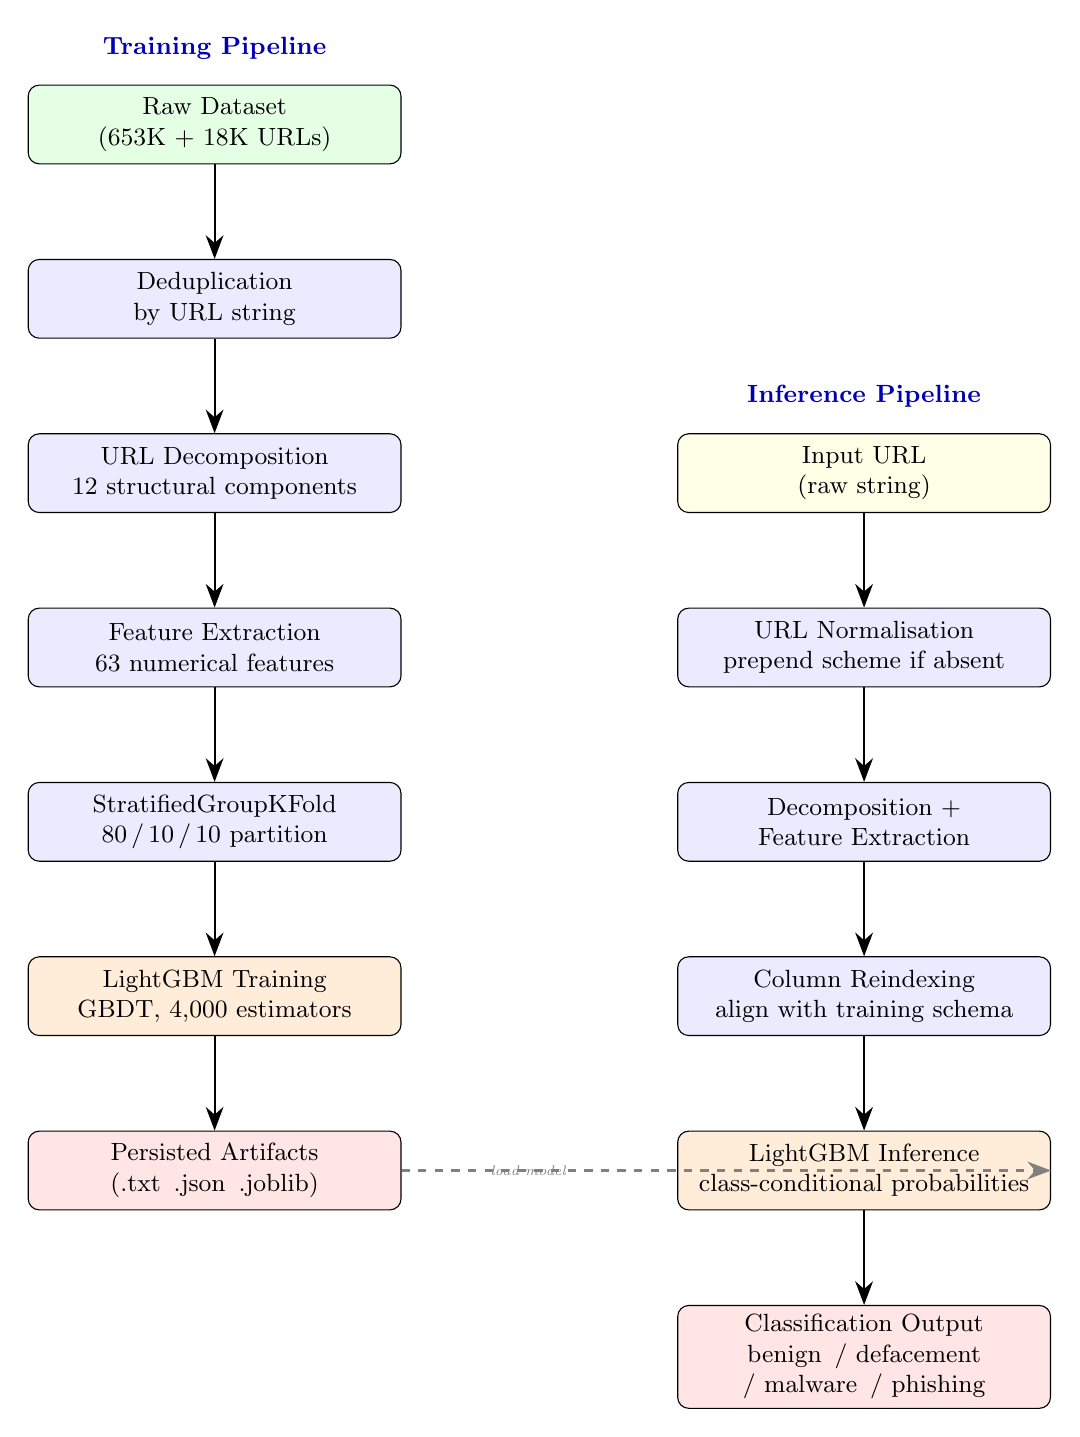
\begin{tikzpicture}[
    node distance=1.2cm and 2cm,
    block/.style={
        rectangle, draw, rounded corners,
        text width=4.5cm, minimum height=1cm,
        align=center, fill=blue!8,
        font=\small
    },
    arrow/.style={-{Stealth[length=3mm]}, thick},
    label/.style={font=\tiny\itshape, text=gray}
]
% ── Training Pipeline (left) ──
\node[block, fill=green!10] (data) {Raw Dataset\\(653K + 18K URLs)};
\node[block, below=of data] (dedup) {Deduplication\\by URL string};
\node[block, below=of dedup] (parse) {URL Decomposition\\12 structural components};
\node[block, below=of parse] (feat) {Feature Extraction\\63 numerical features};
\node[block, below=of feat] (split) {StratifiedGroupKFold\\80\,/\,10\,/\,10 partition};
\node[block, below=of split, fill=orange!15] (train) {LightGBM Training\\GBDT, 4{,}000 estimators};
\node[block, below=of train, fill=red!10] (model) {Persisted Artifacts\\(.txt\enspace .json\enspace .joblib)};

\draw[arrow] (data) -- (dedup);
\draw[arrow] (dedup) -- (parse);
\draw[arrow] (parse) -- (feat);
\draw[arrow] (feat) -- (split);
\draw[arrow] (split) -- (train);
\draw[arrow] (train) -- (model);

% ── Inference Pipeline (right) ──
\node[block, fill=yellow!10, right=3.5cm of parse] (input) {Input URL\\(raw string)};
\node[block, below=of input] (norm) {URL Normalisation\\prepend scheme if absent};
\node[block, below=of norm] (iparse) {Decomposition +\\Feature Extraction};
\node[block, below=of iparse] (reindex) {Column Reindexing\\align with training schema};
\node[block, below=of reindex, fill=orange!15] (predict) {LightGBM Inference\\class-conditional probabilities};
\node[block, below=of predict, fill=red!10] (output) {Classification Output\\benign\enspace / defacement\\/ malware\enspace / phishing};

\draw[arrow] (input) -- (norm);
\draw[arrow] (norm) -- (iparse);
\draw[arrow] (iparse) -- (reindex);
\draw[arrow] (reindex) -- (predict);
\draw[arrow] (predict) -- (output);

% ── Connection ──
\draw[arrow, dashed, gray] (model.east) -- ++(1,0) |- (predict.east)
    node[midway, right, label] {load model};

% ── Labels ──
\node[above=0.2cm of data, font=\bfseries\small, color=blue!70!black] {Training Pipeline};
\node[above=0.2cm of input, font=\bfseries\small, color=blue!70!black] {Inference Pipeline};

\end{tikzpicture}
\caption{High-level architecture of the training and inference pipelines.}
\label{fig:pipeline}
\end{figure}

% ──────────────────────────────────────────────────────────────
\subsection{URL Normalisation}
% ──────────────────────────────────────────────────────────────

Raw URLs in the wild frequently omit the scheme component (e.g., \texttt{example.com/path} rather than \texttt{https://example.com/path}). To ensure consistent parsing, a two-stage normalisation procedure is applied:

\begin{enumerate}
    \item \textbf{Training-time normalisation.} If the URL does not match the pattern \verb|^[a-zA-Z][a-zA-Z0-9+\-.]*://| and does not begin with \texttt{//}, the prefix \texttt{//} is prepended. This enables \texttt{urlparse} to correctly identify the network location without imposing an artificial scheme.
    \item \textbf{Inference-time normalisation.} For user-submitted URLs that lack both a scheme and any path separator (\texttt{/}), the prefix \texttt{https://} is prepended as a sensible default.
\end{enumerate}

\begin{lstlisting}[caption={URL normalisation functions}]
def normalize_url(url: str) -> str:
    """Training-time normalisation."""
    if re.match(r'^[a-zA-Z][a-zA-Z0-9\+\-\.]*://', url):
        return url                    # scheme already present
    if url.startswith('//'):
        return url                    # protocol-relative URL
    return '//' + url                 # prepend // for urlparse

def normalize_input_url(url: str) -> str:
    """Inference-time normalisation."""
    url = url.strip()
    if not re.match(r'^[a-zA-Z][a-zA-Z0-9+\-.]*://', url) \
       and '/' not in url:
        url = 'https://' + url
    return url
\end{lstlisting}

% ──────────────────────────────────────────────────────────────
\subsection{URL Decomposition}
% ──────────────────────────────────────────────────────────────

Each normalised URL is decomposed into 12 structural components through the combined use of Python's \texttt{urllib.parse.urlparse} and the \texttt{tldextract} library~\cite{tldextract}. Table~\ref{tab:url_components} enumerates these components.

\begin{table}[H]
\centering
\caption{The 12 structural components extracted from each URL.}
\label{tab:url_components}
\begin{tabular}{clll}
\toprule
\textbf{Index} & \textbf{Component} & \textbf{Parser} & \textbf{Example} \\
\midrule
0  & Scheme     & \texttt{urlparse}   & \texttt{https} \\
1  & Netloc     & \texttt{urlparse}   & \texttt{user:pass@sub.example.com:8080} \\
2  & Username   & \texttt{urlparse}   & \texttt{user} \\
3  & Password   & \texttt{urlparse}   & \texttt{pass} \\
4  & Port       & \texttt{urlparse}   & \texttt{8080} \\
5  & Subdomain  & \texttt{tldextract} & \texttt{sub} \\
6  & Domain     & \texttt{tldextract} & \texttt{example} \\
7  & Suffix     & \texttt{tldextract} & \texttt{com} \\
8  & Path       & \texttt{urlparse}   & \texttt{/page/index.html} \\
9  & Params     & \texttt{urlparse}   & (RFC~2396 parameters) \\
10 & Query      & \texttt{urlparse}   & \texttt{id=123\&lang=en} \\
11 & Fragment   & \texttt{urlparse}   & \texttt{section-2} \\
\bottomrule
\end{tabular}
\end{table}

All percent-encoded components (e.g., \texttt{\%20}, \texttt{\%3D}) are recursively decoded to their plaintext representation via iterative application of \texttt{urllib.parse.unquote\_plus}:

\begin{lstlisting}[caption={Recursive percent-decoding}]
def fully_decode(data: str) -> str:
    if not data:
        return ""
    current = str(data)
    while True:
        decoded = unquote_plus(current)
        if decoded == current:
            break
        current = decoded
    return current
\end{lstlisting}

% ──────────────────────────────────────────────────────────────
\subsection{Inference Pipeline}
% ──────────────────────────────────────────────────────────────

At inference time, the following procedure is executed for each input URL:

\begin{enumerate}
    \item \textbf{Artifact loading.} The persisted LightGBM Booster (\texttt{.txt}), the label encoder (\texttt{.joblib}), the metadata schema (\texttt{.json}), and the whitelist are loaded into memory.
    \item \textbf{Normalisation.} The input URL is normalised as described above.
    \item \textbf{Feature extraction.} The function \texttt{features\_extraction(url, whitelist)} computes all 63 features.
    \item \textbf{Post-processing.} Raw textual columns (\texttt{scheme}, \texttt{netloc}, \texttt{path}, \texttt{query}, \texttt{fragment}, \texttt{subdomain}, \texttt{domain}) are discarded. The \texttt{url\_length} feature is appended, and the scheme is one-hot encoded into five binary indicators (\texttt{is\_https}, \texttt{is\_http}, \texttt{is\_ftp}, \texttt{is\_none}, \texttt{is\_other}).
    \item \textbf{Column reindexing.} The feature vector is reindexed to match the exact column ordering used during training, as recorded in the metadata file.
    \item \textbf{Prediction.} The LightGBM Booster returns a probability vector $\mathbf{p} \in \mathbb{R}^4$, one entry per class.
    \item \textbf{Label mapping.} Probabilities are mapped to human-readable class names via the persisted label encoder.
\end{enumerate}

\begin{lstlisting}[caption={Core inference logic}]
def predict_url(url, booster, le, feature_columns, whitelist):
    X_row = url_to_feature_row(url, feature_columns, whitelist)
    proba = booster.predict(X_row)[0]
    labels = le if isinstance(le, np.ndarray) else le.classes_
    result = {label: round(float(p) * 100, 2)
              for label, p in zip(labels, proba)}
    return result
\end{lstlisting}

% ==============================================================
\section{Feature Engineering}
\label{sec:features}
% ==============================================================

A total of \textbf{63 numerical features} are extracted from each URL, organised into six thematically coherent groups. This section provides an exhaustive specification of every feature, its computational definition, and its security rationale. The feature engineering stage constitutes the core intellectual contribution of the system and is the primary determinant of classification performance.

% ──────────────────────────────────────────────────────────────
\subsection{Group~1: Structural and Presence Features \texorpdfstring{$(n=14)$}{(n=14)}}
\label{sec:feat_structural}
% ──────────────────────────────────────────────────────────────

This group captures the macro-level composition of the URL by encoding the presence or absence of each structural component and the overall complexity of the URL.

\begin{longtable}{p{4.5cm}p{1.5cm}p{7cm}}
\toprule
\textbf{Feature} & \textbf{Type} & \textbf{Description} \\
\midrule
\endhead
\texttt{url\_length}       & int   & Total character length of the raw URL string. Malicious URLs---particularly those embedding encoded payloads---tend to exhibit anomalously high lengths. \\
\texttt{number\_of\_part}  & int   & Count of non-empty URL components among \{scheme, netloc, path, query, fragment\}. Values range from 0 to 5. \\
\texttt{has\_scheme}       & bin   & Indicates whether a scheme (e.g., \texttt{http}, \texttt{https}, \texttt{ftp}) is explicitly specified. \\
\texttt{has\_netloc}       & bin   & Indicates the presence of the network location component. \\
\texttt{has\_path}         & bin   & Indicates the presence of a path component. \\
\texttt{has\_params}       & bin   & Indicates the presence of RFC~2396 path parameters. \\
\texttt{has\_query}        & bin   & Indicates the presence of a query string. \\
\texttt{has\_fragment}     & bin   & Indicates the presence of a fragment identifier. \\
\texttt{has\_username}     & bin   & Indicates whether the URL embeds a username in the authority component. This is a well-documented phishing vector, as browsers may display the embedded credentials as if they were part of the domain. \\
\texttt{has\_password}     & bin   & Indicates the presence of an embedded password in the authority component. \\
\texttt{has\_port}         & bin   & Indicates whether an explicit port number is specified. \\
\texttt{has\_subdomain}    & bin   & Indicates the presence of a subdomain (extracted via \texttt{tldextract}). \\
\texttt{has\_domain}       & bin   & Indicates whether a valid registered domain is present. \\
\texttt{has\_suffix}       & bin   & Indicates the presence of a recognised top-level domain (TLD) suffix. \\
\bottomrule
\caption{Group~1: Structural and Presence Features.}
\label{tab:structural}
\end{longtable}

\textbf{Security rationale.} Phishing URLs frequently embed credentials within the netloc to deceive users (e.g., \texttt{http://paypal.com@evil.com/login}). Malware distribution URLs in the training corpus overwhelmingly specify an explicit scheme, whereas benign URLs harvested from domain lists often omit the scheme.

% ──────────────────────────────────────────────────────────────
\subsection{Group~2: Length Features \texorpdfstring{$(n=6)$}{(n=6)}}
\label{sec:feat_length}
% ──────────────────────────────────────────────────────────────

This group measures the character length of individual URL components. Anomalously long components may indicate obfuscated payloads, excessively deep directory structures, or inflated query strings.

\begin{longtable}{p{4.5cm}p{1.5cm}p{7cm}}
\toprule
\textbf{Feature} & \textbf{Type} & \textbf{Description} \\
\midrule
\endhead
\texttt{netloc\_length}     & int & Character length of the network location. \\
\texttt{path\_length}       & int & Character length of the path component. \\
\texttt{query\_length}      & int & Character length of the query string. \\
\texttt{fragment\_length}   & int & Character length of the fragment identifier. \\
\texttt{subdomain\_length}  & int & Character length of the subdomain. \\
\texttt{domain\_length}     & int & Character length of the registered domain. \\
\bottomrule
\caption{Group~2: Length Features.}
\label{tab:length}
\end{longtable}

% ──────────────────────────────────────────────────────────────
\subsection{Group~3: Statistical and Entropy Features \texorpdfstring{$(n=6)$}{(n=6)}}
\label{sec:feat_entropy}
% ──────────────────────────────────────────────────────────────

Shannon entropy~\cite{shannon} quantifies the degree of randomness within a character sequence. Algorithmically generated domains (AGDs) and machine-generated paths---commonly employed by malware and C2 infrastructure---exhibit characteristically elevated entropy relative to human-authored strings.

The Shannon entropy of a string $s$ of length $n$ with character frequency counts $\{c_1, c_2, \ldots, c_k\}$ is computed as:

\begin{equation}
H(s) = \log_2(n) - \frac{1}{n}\sum_{i=1}^{k} c_i \cdot \log_2(c_i)
\label{eq:entropy}
\end{equation}

\begin{longtable}{p{4.5cm}p{1.5cm}p{7cm}}
\toprule
\textbf{Feature} & \textbf{Type} & \textbf{Description} \\
\midrule
\endhead
\texttt{url\_entropy}       & float & Shannon entropy computed over the entire URL string. \\
\texttt{netloc\_entropy}    & float & Shannon entropy of the network location. \\
\texttt{path\_entropy}      & float & Shannon entropy of the path component. \\
\texttt{query\_entropy}     & float & Shannon entropy of the query string. \\
\texttt{subdomain\_entropy} & float & Shannon entropy of the subdomain. \\
\texttt{domain\_entropy}    & float & Shannon entropy of the registered domain. \\
\bottomrule
\caption{Group~3: Statistical and Entropy Features.}
\label{tab:entropy}
\end{longtable}

\begin{lstlisting}[caption={Shannon entropy implementation}]
def Shannon_entropy(data: str) -> float:
    if not data:
        return 0
    char_count = Counter(data)
    n = len(data)
    s = sum(c * log2(c) for c in char_count.values())
    return log2(n) - s / n
\end{lstlisting}

% ──────────────────────────────────────────────────────────────
\subsection{Group~4: Special Character Features \texorpdfstring{$(n=11)$}{(n=11)}}
\label{sec:feat_special}
% ──────────────────────────────────────────────────────────────

This group quantifies the occurrence of specific punctuation and non-alphanumeric characters within designated URL components. Certain character patterns serve as strong discriminative signals: for instance, the presence of the \texttt{@} symbol in the netloc is a well-known URL spoofing technique, and an elevated hyphen count in the subdomain is characteristic of phishing domains (e.g., \texttt{secure-login-paypal.attacker.com}).

\begin{longtable}{p{5.2cm}p{1.3cm}p{6.5cm}}
\toprule
\textbf{Feature} & \textbf{Type} & \textbf{Description} \\
\midrule
\endhead
\texttt{hyphen\_in\_subdomain} & int & Count of hyphen characters (\texttt{-}) in the subdomain. Phishing campaigns frequently construct multi-word subdomains mimicking trusted brands. \\
\texttt{hyphen\_in\_domain}    & int & Count of hyphen characters in the registered domain. \\
\texttt{unicode}               & bin & Indicates whether the domain contains non-ASCII characters (codepoints $> 127$). This is indicative of Internationalised Domain Name (IDN) homograph attacks. \\
\texttt{punycode}              & bin & Indicates the presence of the \texttt{xn--} prefix, signalling Punycode-encoded internationalised domain names. \\
\texttt{at\_sign\_in\_netloc}  & int & Count of \texttt{@} characters in the netloc. This character can redirect the browser to a different host (e.g., \texttt{http://trusted.com@evil.com}). \\
\texttt{slash\_in\_path}       & int & Count of forward slashes (\texttt{/}) in the path, reflecting directory depth. \\
\texttt{dot\_in\_path}         & int & Count of dots (\texttt{.}) in the path, often corresponding to file extensions. \\
\texttt{strange\_in\_query}    & int & Count of characters outside the RFC~3986 unreserved and reserved character sets. \\
\texttt{equal\_in\_query}      & int & Count of equals signs (\texttt{=}) in the query string, approximating the number of key-value parameter pairs. \\
\texttt{ampersand\_in\_query}  & int & Count of ampersand characters (\texttt{\&}) in the query string. \\
\texttt{number\_subdomain}     & int & Number of subdomain levels, computed as the dot count within the subdomain plus one. \\
\bottomrule
\caption{Group~4: Special Character Features.}
\label{tab:special_char}
\end{longtable}

Characters deemed ``strange'' are identified via a regular expression that matches any character not belonging to the RFC~3986 standard character set:

\begin{lstlisting}[caption={Non-standard character detection pattern (RFC 3986 complement)}]
STRANGE_CHAR_PATTERN = re.compile(
    r"[^a-zA-Z0-9\-\._~:/\?#\[\]@!\$&'\(\)\*\+,;=%]"
)
\end{lstlisting}

% ──────────────────────────────────────────────────────────────
\subsection{Group~5: Lexical and Heuristic Features \texorpdfstring{$(n=16)$}{(n=16)}}
\label{sec:feat_lexical}
% ──────────────────────────────────────────────────────────────

This group constitutes the most analytically complex feature category, employing string-similarity algorithms, phonotactic heuristics, and keyword-based threat indicators.

\begin{longtable}{p{5.8cm}p{1.2cm}p{6cm}}
\toprule
\textbf{Feature} & \textbf{Type} & \textbf{Description} \\
\midrule
\endhead
\texttt{normalized\_levenshtein\_domain} & float &
    Normalised Levenshtein similarity between the host domain and the closest match in the whitelist (see Section~\ref{sec:levenshtein}). Elevated values indicate potential brand impersonation. \\
\texttt{normalized\_levenshtein\_subdomain} & float &
    Analogous computation applied to the subdomain component. \\
\texttt{random\_domain\_check} & float &
    Consonant-to-letter ratio in the domain. Algorithmically generated domains (AGDs) tend to exhibit a higher consonant density than natural-language domains. \\
\texttt{random\_subdomain\_check} & float &
    Consonant ratio computed for the subdomain. \\
\texttt{number\_ratio\_domain} & float &
    Proportion of digit characters within the domain string. Legitimate domains rarely consist predominantly of digits. \\
\texttt{number\_ratio\_subdomain} & float &
    Digit proportion in the subdomain. \\
\texttt{repeated\_domain\_check} & float &
    Ratio of adjacent identical character pairs to total character transitions in the domain. \\
\texttt{repeated\_path\_check} & float &
    Adjacent character repetition ratio in the path. \\
\texttt{repeated\_url\_check} & float &
    Adjacent character repetition ratio across the entire URL. \\
\texttt{longest\_repeated\_chain} & int &
    Length of the longest contiguous run of a single repeated character in the URL. \\
\texttt{ip\_domain} & bin &
    Indicates whether the domain component is a valid IPv4 or IPv6 address rather than a textual hostname. IP-literal domains are frequently used by malware to bypass domain-based blacklists. \\
\texttt{suspicious\_key\_domain} & bin &
    Indicates whether the domain contains any suspicious keyword (see Table~\ref{tab:keywords}). \\
\texttt{suspicious\_key\_subdomain} & bin &
    Suspicious keyword presence in the subdomain. \\
\texttt{suspicious\_key\_path} & bin &
    Suspicious keyword presence in the path. \\
\texttt{suspicious\_key\_query} & bin &
    Suspicious keyword presence in the query string. \\
\texttt{shortened} & bin &
    Indicates whether the URL uses a known URL shortening service (e.g., \texttt{bit.ly}, \texttt{goo.gl}, \texttt{tinyurl.com}). \\
\bottomrule
\caption{Group~5: Lexical and Heuristic Features.}
\label{tab:lexical}
\end{longtable}

% ── Levenshtein subsection ────────────────────────────────────
\subsubsection{Levenshtein Similarity with the Whitelist}
\label{sec:levenshtein}

The normalised Levenshtein similarity is the single most discriminative feature for phishing detection. For each input URL, the host domain $d$ is compared against all 10,001 entries in the trusted domain whitelist $W$. The algorithm employs two optimisation strategies to reduce the computational cost from $O(|W| \cdot |d|^2)$: (i)~a \textit{length pre-filter} that skips whitelist entries whose length difference exceeds a dynamic threshold, and (ii)~the \texttt{score\_cutoff} parameter of the RapidFuzz~\cite{rapidfuzz} library, which enables early termination of the distance computation.

\begin{algorithm}[H]
\caption{Optimised Levenshtein similarity against the whitelist.}
\label{alg:levenshtein}
\begin{algorithmic}[1]
\Require Domain string $d$; whitelist $W = \{w_1, w_2, \ldots, w_{|W|}\}$
\Ensure Normalised similarity score $s^* \in [0, 1]$
\State $\tau \gets \max\!\bigl(1,\; \lfloor |d|\,/\,7 \rfloor\bigr)$ \Comment{Dynamic edit-distance threshold}
\State $s^* \gets 0$
\For{each $w \in W$}
    \If{$\bigl||d| - |w|\bigr| > \tau$} \textbf{continue} \Comment{Length pre-filter}
    \EndIf
    \State $\delta \gets \mathrm{Levenshtein.distance}(d,\, w,\, \mathrm{cutoff}{=}\tau)$
    \If{$\delta \leq \tau$}
        \State $s \gets \mathrm{Levenshtein.normalized\_similarity}(d,\, w)$
        \If{$s > s^*$}
            \State $s^* \gets s;\quad w^* \gets w$
        \EndIf
    \EndIf
\EndFor
\State \Return $s^*$
\end{algorithmic}
\end{algorithm}

\textbf{Dynamic threshold rationale.} The threshold $\tau = \max(1, \lfloor |d|/7 \rfloor)$ scales with domain length: short domains (e.g., \texttt{fb.com}) permit at most one edit, while longer domains allow proportionally more edits. This prevents false-positive similarity matches on short strings.

% ── Suspicious keywords ──────────────────────────────────────
\subsubsection{Suspicious Keyword Taxonomy}

The system maintains a curated lexicon of over 40 keywords, organised by semantic category, that are frequently observed in phishing and social engineering URLs.

\begin{table}[H]
\centering
\caption{Suspicious keyword categories and representative terms.}
\label{tab:keywords}
\begin{tabular}{ll}
\toprule
\textbf{Category} & \textbf{Representative Keywords} \\
\midrule
Authentication & \texttt{login}, \texttt{signin}, \texttt{sign-in}, \texttt{log-in}, \texttt{logout} \\
Account        & \texttt{account}, \texttt{myaccount}, \texttt{profile}, \texttt{user} \\
Security       & \texttt{secure}, \texttt{verify}, \texttt{validate}, \texttt{confirm} \\
Financial      & \texttt{banking}, \texttt{payment}, \texttt{checkout}, \texttt{billing}, \texttt{wallet} \\
Urgency        & \texttt{update}, \texttt{urgent}, \texttt{alert}, \texttt{warning}, \texttt{suspend} \\
Support        & \texttt{support}, \texttt{helpdesk}, \texttt{recover}, \texttt{reset}, \texttt{password} \\
Webmail        & \texttt{webmail}, \texttt{outlook}, \texttt{office365}, \texttt{cpanel} \\
\bottomrule
\end{tabular}
\end{table}

% ──────────────────────────────────────────────────────────────
\subsection{Group~6: Advanced Cyber Threat Indicators \texorpdfstring{$(n=10)$}{(n=10)}}
\label{sec:feat_advanced}
% ──────────────────────────────────────────────────────────────

This final group targets specific threat vectors that have been empirically observed in real-world malware distribution and phishing campaigns.

\begin{longtable}{p{4.8cm}p{1.3cm}p{6.9cm}}
\toprule
\textbf{Feature} & \textbf{Type} & \textbf{Description and Threat Model} \\
\midrule
\endhead
\texttt{has\_uuid\_path} & bin &
    Detects the presence of a UUID-formatted string (pattern: \texttt{[0-9a-f]\{8\}-[0-9a-f]\{4\}-...-[0-9a-f]\{12\}}) within the URL path. UUIDs in paths are a hallmark of C2 server callback channels and automated malware staging. \\
\texttt{download\_param} & bin &
    Indicates whether the path or query string contains the substrings \texttt{download} or \texttt{install} (applicable only when the respective component exceeds 7~characters in length). This feature targets drive-by download vectors. \\
\texttt{free\_host} & bin &
    Indicates whether the domain belongs to a known free hosting platform (e.g., \texttt{vercel.app}, \texttt{netlify.app}, \texttt{github.io}, \texttt{000webhostapp.com}). Adversaries frequently exploit free hosting services due to their zero-cost, rapid provisioning, and perceived trustworthiness. \\
\texttt{free\_host\_download} & bin &
    Conjunction of \texttt{free\_host} and \texttt{download\_param}. This composite feature provides an exceptionally strong signal for malware distribution via free hosting infrastructure. \\
\texttt{suspicious\_suffix} & bin &
    Indicates whether the TLD belongs to a curated set of 30 TLDs that are disproportionately associated with abuse (e.g., \texttt{.tk}, \texttt{.ml}, \texttt{.ga}, \texttt{.cf}, \texttt{.xyz}, \texttt{.top}, \texttt{.click}). \\
\texttt{is\_https} & bin & Scheme is \texttt{https}. \\
\texttt{is\_http}  & bin & Scheme is \texttt{http}. \\
\texttt{is\_ftp}   & bin & Scheme is \texttt{ftp}. \\
\texttt{is\_none}  & bin & No scheme is present. \\
\texttt{is\_other} & bin & Scheme is not one of \texttt{http/https/ftp} and is not empty (e.g., \texttt{data:}, \texttt{javascript:}). \\
\bottomrule
\caption{Group~6: Advanced Cyber Threat Indicators.}
\label{tab:advanced}
\end{longtable}

\textbf{Suspicious TLD set.} The following 30 TLDs are flagged based on empirical abuse prevalence data:

\begin{lstlisting}[caption={Set of suspicious top-level domains}]
SUSPICIOUS_TLDS = {
    'tk', 'ml', 'ga', 'cf', 'gq', 'xyz', 'top', 'click',
    'link', 'win', 'download', 'racing', 'vip', 'club',
    'online', 'site', 'live', 'fun', 'space', 'pw',
    'christmas', 'cyou', 'rest', 'icu', 'cfd', 'hair',
    'makeup', 'monster', 'quest', 'skin',
}
\end{lstlisting}

\textbf{Free hosting services.} The following 15 hosting platforms are monitored:

\begin{lstlisting}[caption={Set of monitored free hosting domains}]
FREE_HOSTING = {
    'vercel.app', 'netlify.app', 'github.io', 'glitch.me',
    'replit.dev', 'repl.co', '000webhostapp.com', 'web.app',
    'firebaseapp.com', 'pages.dev', 'surge.sh', 'onrender.com',
    'railway.app', 'fly.dev', 'cyclic.app'
}
\end{lstlisting}

% ──────────────────────────────────────────────────────────────
\subsection{Feature Summary}
% ──────────────────────────────────────────────────────────────

\begin{table}[H]
\centering
\caption{Summary of the six feature groups.}
\label{tab:feat_summary}
\begin{tabular}{clc}
\toprule
\textbf{Group} & \textbf{Category} & \textbf{Count} \\
\midrule
1 & Structural \& Presence       & 14 \\
2 & Length                        & 6 \\
3 & Statistical \& Entropy       & 6 \\
4 & Special Characters            & 11 \\
5 & Lexical \& Heuristic          & 16 \\
6 & Advanced Threat Indicators    & 10 \\
\midrule
  & \textbf{Total}                & \textbf{63} \\
\bottomrule
\end{tabular}
\end{table}

% ==============================================================
\section{Model Training}
\label{sec:training}
% ==============================================================

% ──────────────────────────────────────────────────────────────
\subsection{Data Preprocessing}
% ──────────────────────────────────────────────────────────────

\subsubsection{Label Encoding}

The four string-valued class labels are transformed into integer codes via \texttt{sklearn.preprocessing.LabelEncoder}:

\begin{table}[H]
\centering
\caption{Label encoding mapping.}
\begin{tabular}{cl}
\toprule
\textbf{Code} & \textbf{Class} \\
\midrule
0 & benign \\
1 & defacement \\
2 & malware \\
3 & phishing \\
\bottomrule
\end{tabular}
\end{table}

\subsubsection{Feature Matrix Construction}

The feature matrix $\mathbf{X} \in \mathbb{R}^{N \times 63}$ is constructed by retaining only the 63 numerical features and discarding all raw textual columns:

\begin{lstlisting}[caption={Feature matrix construction}]
RAW_TEXT_COLUMNS = {"url", "type", "scheme", "netloc", "path",
                    "query", "fragment", "subdomain", "domain"}
X = df.drop(columns=RAW_TEXT_COLUMNS)
y = df['type']
\end{lstlisting}

\subsubsection{Deduplication}

Prior to partitioning, all exact-duplicate URLs are removed to prevent information leakage through replicated samples:

\begin{lstlisting}[caption={Deduplication}]
url_data = url_data.drop_duplicates(subset='url').reset_index(drop=True)
\end{lstlisting}

% ──────────────────────────────────────────────────────────────
\subsection{Data Partitioning via Stratified Group $K$-Fold}
\label{sec:split}
% ──────────────────────────────────────────────────────────────

A na\"{i}ve random split (e.g., \texttt{train\_test\_split}) introduces a subtle but significant form of data leakage: URLs sharing the same registered domain (e.g., \texttt{example.com/page1} and \texttt{example.com/page2}) may be distributed across both the training and test sets. The model can then exploit domain-level memorisation rather than learning generalisable URL-level patterns, resulting in inflated evaluation metrics that do not reflect true out-of-distribution performance.

To address this, we employ \texttt{sklearn.model\_selection.StratifiedGroupKFold} with $K{=}10$ folds, using the registered domain as the grouping variable:

\begin{lstlisting}[caption={Stratified Group $K$-Fold partitioning}]
from sklearn.model_selection import StratifiedGroupKFold

sgkf = StratifiedGroupKFold(n_splits=10, shuffle=True,
                             random_state=36)
folds = list(sgkf.split(X, y, groups=url_data['domain']))

test_idx  = folds[0][1]                                 # ~10%
val_idx   = folds[1][1]                                  # ~10%
train_idx = np.concatenate([folds[i][1] for i in range(2, 10)])  # ~80%
\end{lstlisting}

This partitioning strategy guarantees the following invariants:
\begin{itemize}
    \item \textbf{Stratification.} The class distribution within each fold is approximately proportional to the overall dataset distribution.
    \item \textbf{Group integrity.} All URLs belonging to the same registered domain are confined to a single fold, yielding \textbf{zero domain overlap} between the training, validation, and test sets.
\end{itemize}

\begin{table}[H]
\centering
\caption{Data partition statistics.}
\label{tab:split}
\begin{tabular}{lrr}
\toprule
\textbf{Partition} & \textbf{Samples} & \textbf{Proportion} \\
\midrule
Training   & 529,580 & 80\% \\
Validation &  66,198 & 10\% \\
Test       &  66,198 & 10\% \\
\midrule
\textbf{Total} & \textbf{661,976} & \textbf{100\%} \\
\bottomrule
\end{tabular}
\end{table}

% ──────────────────────────────────────────────────────────────
\subsection{LightGBM Hyperparameter Configuration}
\label{sec:hyperparams}
% ──────────────────────────────────────────────────────────────

The classifier is implemented using the LightGBM~\cite{lightgbm} framework with the Gradient Boosted Decision Trees (GBDT) algorithm. Table~\ref{tab:hyperparams} presents the complete hyperparameter specification.

\begin{table}[H]
\centering
\caption{LightGBM hyperparameter configuration.}
\label{tab:hyperparams}
\begin{tabular}{llp{6.2cm}}
\toprule
\textbf{Parameter} & \textbf{Value} & \textbf{Rationale} \\
\midrule
\multicolumn{3}{l}{\textit{Objective and Task}} \\
\texttt{objective}       & \texttt{multiclass}  & Multi-class softmax cross-entropy loss. \\
\texttt{num\_class}      & 4           & Four target classes. \\
\texttt{boosting\_type}  & \texttt{gbdt}        & Gradient Boosted Decision Trees. \\
\texttt{class\_weight}   & \texttt{balanced}    & Inversely proportional to class frequency. \\
\midrule
\multicolumn{3}{l}{\textit{Capacity Control}} \\
\texttt{n\_estimators}       & 4{,}000 & Maximum number of boosting rounds. \\
\texttt{learning\_rate}      & 0.025   & Conservative step size to promote generalisation. \\
\texttt{max\_depth}          & 5       & Maximum tree depth. \\
\texttt{num\_leaves}         & 24      & Maximum leaf count per tree ($< 2^5 = 32$). \\
\texttt{min\_data\_in\_leaf} & 50      & Minimum samples per leaf node. \\
\midrule
\multicolumn{3}{l}{\textit{Stochastic Subsampling}} \\
\texttt{colsample\_bytree} & 0.75 & Feature subsampling rate per tree. \\
\texttt{subsample}         & 0.80 & Row subsampling rate per boosting round. \\
\texttt{subsample\_freq}   & 1    & Subsampling applied at every iteration. \\
\midrule
\multicolumn{3}{l}{\textit{Regularisation}} \\
\texttt{reg\_alpha}           & 0.1  & $\ell_1$ (Lasso) regularisation coefficient. \\
\texttt{reg\_lambda}          & 1.0  & $\ell_2$ (Ridge) regularisation coefficient. \\
\texttt{min\_gain\_to\_split} & 0.01 & Minimum information gain required to perform a split. \\
\midrule
\multicolumn{3}{l}{\textit{Early Stopping}} \\
\texttt{early\_stopping\_rounds} & 100 & Training halts if the validation loss fails to improve for 100 consecutive rounds. \\
\bottomrule
\end{tabular}
\end{table}

% ──────────────────────────────────────────────────────────────
\subsection{Training Procedure}
\label{sec:train_procedure}
% ──────────────────────────────────────────────────────────────

The model is trained using the scikit-learn--compatible \texttt{LGBMClassifier} interface. Two evaluation metrics are monitored concurrently: the primary \texttt{multi\_logloss} (multiclass cross-entropy) and the secondary \texttt{auc\_mu} (multiclass area under the ROC curve). Training progress is logged at 100-iteration intervals.

\begin{lstlisting}[caption={LightGBM training procedure}]
model = lgb.LGBMClassifier(**params)

callbacks = [
    lgb.early_stopping(stopping_rounds=100, verbose=True),
    lgb.log_evaluation(100)
]

model.fit(
    X_train, y_train,
    eval_set=[(X_train, y_train), (X_val, y_val)],
    eval_names=['train', 'val'],
    callbacks=callbacks,
    eval_metric=['multi_logloss', 'auc_mu']
)
\end{lstlisting}

\textbf{Training outcome.} Early stopping was triggered at \textbf{iteration~738} out of a maximum of 4,000 rounds, indicating that the model achieved convergence well within the allocated capacity. The relatively early termination---at 18.5\% of the maximum budget---suggests that the combination of a conservative learning rate ($\eta = 0.025$) and 4,000 estimators provides ample capacity for this classification task.

% ──────────────────────────────────────────────────────────────
\subsection{Evaluation Results}
\label{sec:results}
% ──────────────────────────────────────────────────────────────

The trained model is evaluated on the held-out test partition (66,198 samples) with \textbf{zero domain overlap} with the training set.

\begin{itemize}
    \item \textbf{Test Accuracy:} \textbf{93.46\%}
    \item \textbf{Evaluation Metrics:} Per-class precision, recall, and $F_1$-score via \texttt{classification\_report}.
    \item \textbf{Visual Diagnostics:} Confusion matrix and train/validation learning curves (\texttt{multi\_logloss} over iterations).
    \item \textbf{Model Interpretability:} Feature importance (information gain) and SHAP~(SHapley Additive exPlanations) value analysis.
\end{itemize}

% ==============================================================
\section{Model Architecture}
\label{sec:architecture}
% ==============================================================

% ──────────────────────────────────────────────────────────────
\subsection{Gradient Boosted Decision Trees}
% ──────────────────────────────────────────────────────────────

LightGBM~\cite{lightgbm} implements a highly optimised variant of Gradient Boosted Decision Trees (GBDT), originally proposed by Friedman~(2001). The ensemble prediction for a sample $\mathbf{x}_i$ is given by:

\begin{equation}
\hat{y}_i = \sum_{t=1}^{T} \eta \cdot f_t(\mathbf{x}_i)
\label{eq:gbdt}
\end{equation}

\noindent where $T$ denotes the number of boosting rounds ($T = 738$ after early stopping), $f_t$ is the $t$-th regression tree, and $\eta = 0.025$ is the learning rate (shrinkage parameter).

Key algorithmic innovations in LightGBM that contribute to its computational efficiency include \textit{Gradient-based One-Side Sampling} (GOSS), which retains samples with large gradients while randomly sampling those with small gradients, and \textit{Exclusive Feature Bundling} (EFB), which bundles mutually exclusive features to reduce the effective feature dimensionality.

% ──────────────────────────────────────────────────────────────
\subsection{Objective Function}
% ──────────────────────────────────────────────────────────────

For the four-class classification task, the objective function is the softmax cross-entropy loss:

\begin{equation}
\mathcal{L} = -\frac{1}{N}\sum_{i=1}^{N}\sum_{c=1}^{C} y_{i,c} \cdot \log\bigl(p_{i,c}\bigr)
\label{eq:loss}
\end{equation}

\noindent where $C = 4$ is the number of classes, $y_{i,c} \in \{0, 1\}$ is the ground-truth indicator, and the class-conditional probability is obtained via the softmax function:

\begin{equation}
p_{i,c} = \frac{\exp(z_{i,c})}{\sum_{j=1}^{C} \exp(z_{i,j})}
\label{eq:softmax}
\end{equation}

\noindent with $z_{i,c}$ denoting the raw logit output for sample $i$ and class $c$.

% ──────────────────────────────────────────────────────────────
\subsection{Class Balancing}
% ──────────────────────────────────────────────────────────────

The \texttt{class\_weight='balanced'} parameter automatically adjusts the sample weight for each class according to:

\begin{equation}
w_c = \frac{N}{C \cdot N_c}
\label{eq:balance}
\end{equation}

\noindent where $N$ is the total number of training samples and $N_c$ is the number of samples belonging to class $c$. This inversely proportional weighting scheme prevents the model from developing a systematic bias toward the majority class.

% ──────────────────────────────────────────────────────────────
\subsection{Multi-Layer Regularisation Strategy}
% ──────────────────────────────────────────────────────────────

To mitigate overfitting, the system employs a six-layer regularisation strategy:

\begin{enumerate}
    \item \textbf{Structural constraints:} $\texttt{max\_depth} = 5$ and $\texttt{num\_leaves} = 24$ limit the representational capacity of individual trees.
    \item \textbf{Minimum leaf population:} $\texttt{min\_data\_in\_leaf} = 50$ prevents the creation of highly specific leaf nodes.
    \item \textbf{Feature subsampling:} $\texttt{colsample\_bytree} = 0.75$ introduces stochasticity by selecting a random subset of features for each tree.
    \item \textbf{Row subsampling:} $\texttt{subsample} = 0.80$ introduces additional randomness through bagging-style sample selection at each iteration.
    \item \textbf{Explicit regularisation:} $\ell_1$ ($\alpha = 0.1$) and $\ell_2$ ($\lambda = 1.0$) penalties on the leaf weights.
    \item \textbf{Minimum split gain:} $\texttt{min\_gain\_to\_split} = 0.01$ suppresses splits that yield negligible information gain.
\end{enumerate}

% ==============================================================
\section{Model Persistence and Artifacts}
\label{sec:artifacts}
% ==============================================================

Upon completion of training, the model and its associated metadata are serialised into four files, enabling reproducible inference without retraining:

\begin{table}[H]
\centering
\caption{Persisted model artifacts.}
\label{tab:artifacts}
\begin{tabular}{llp{6cm}}
\toprule
\textbf{File} & \textbf{Format} & \textbf{Contents} \\
\midrule
\texttt{lgb\_url\_classifier.txt} & LightGBM text & Serialised tree ensemble; loadable via \texttt{lgb.Booster(model\_file=...)}. \\
\texttt{lgb\_url\_classifier.pkl} & Pickle & Full scikit-learn--compatible model object. \\
\texttt{lgb\_url\_classifier\_metadata.json} & JSON & Hyperparameters, ordered feature names, class labels, test accuracy, and training timestamp. \\
\texttt{label\_encoder.joblib} & Joblib & NumPy array of class names for integer-to-label mapping. \\
\bottomrule
\end{tabular}
\end{table}

The metadata file is particularly critical for inference correctness, as it encodes the exact column ordering expected by the model. Any permutation of the feature vector would yield erroneous predictions.

% ==============================================================
\section{Conclusion}
\label{sec:conclusion}
% ==============================================================

This report has presented a complete malicious URL classification system that achieves strong empirical performance through the synergy of principled feature engineering and gradient boosted tree classification. The principal contributions and findings are summarised as follows:

\begin{itemize}
    \item A test accuracy of \textbf{93.46\%} is attained on a held-out partition with \textbf{zero domain overlap} with the training set, providing a rigorous lower bound on the model's generalisation capability.
    \item A comprehensive feature engineering framework comprising \textbf{63 handcrafted features} across six thematic groups---spanning structural, statistical, lexical, and threat-specific dimensions---enables effective classification without any network-level or content-level signals.
    \item The adoption of \textbf{Stratified Group $K$-Fold} partitioning eliminates domain-level data leakage, a pervasive yet frequently overlooked confound in URL classification benchmarks.
    \item The \textbf{LightGBM GBDT} classifier, equipped with a six-layer regularisation strategy, converges at iteration~738 out of 4,000, demonstrating efficient utilisation of model capacity.
    \item The inference pipeline operates entirely on the URL string with \textbf{sub-millisecond latency}, making it suitable for real-time deployment in network security appliances and browser extensions.
\end{itemize}

\subsection{Limitations and Future Work}

Several avenues for improvement merit investigation:

\begin{enumerate}
    \item \textbf{Hyperparameter optimisation.} Systematic tuning via Bayesian optimisation (e.g., Optuna) or random search may yield further performance gains.
    \item \textbf{Ensemble methods.} Combining LightGBM with complementary classifiers such as XGBoost or Random Forest through weighted averaging or stacking may improve robustness.
    \item \textbf{Feature augmentation.} Incorporating WHOIS registration age, SSL certificate attributes, and passive DNS metadata could enhance discriminative power, albeit at the cost of increased inference latency.
    \item \textbf{Dynamic thresholding.} Adapting the classification decision boundary based on contextual signals (e.g., geographic origin, time of day) could improve precision in deployment-specific scenarios.
    \item \textbf{Deployment.} Integration into a REST API or browser extension would enable real-time URL screening for end users.
\end{enumerate}

% ==============================================================
% References
% ==============================================================
\newpage
\begin{thebibliography}{9}

\bibitem{lightgbm}
Ke, G., Meng, Q., Finley, T., Wang, T., Chen, W., Ma, W., Ye, Q., \& Liu, T.-Y. (2017).
\textit{LightGBM: A Highly Efficient Gradient Boosting Decision Tree}.
Advances in Neural Information Processing Systems~30 (NeurIPS), 3149--3157.

\bibitem{tldextract}
Kurkowski, J.
\textit{tldextract --- Accurately separate the TLD from the registered domain and subdomains of a URL}.
\url{https://github.com/john-googling/tldextract}

\bibitem{rapidfuzz}
Bachmann, M.
\textit{RapidFuzz --- Rapid fuzzy string matching in Python and C++}.
\url{https://github.com/maxbachmann/RapidFuzz}

\bibitem{urlhaus}
abuse.ch.
\textit{URLhaus --- Malware URL exchange}.
\url{https://urlhaus.abuse.ch/}

\bibitem{shannon}
Shannon, C.~E. (1948).
A Mathematical Theory of Communication.
\textit{Bell System Technical Journal}, 27(3), 379--423.

\bibitem{levenshtein}
Levenshtein, V.~I. (1966).
Binary codes capable of correcting deletions, insertions, and reversals.
\textit{Soviet Physics Doklady}, 10(8), 707--710.

\bibitem{sklearn}
Pedregosa, F., Varoquaux, G., Gramfort, A., Michel, V., Thirion, B., Grisel, O., \ldots \& Duchesnay, \'E. (2011).
Scikit-learn: Machine Learning in Python.
\textit{Journal of Machine Learning Research}, 12, 2825--2830.

\bibitem{friedman}
Friedman, J.~H. (2001).
Greedy Function Approximation: A Gradient Boosting Machine.
\textit{Annals of Statistics}, 29(5), 1189--1232.

\bibitem{shap}
Lundberg, S.~M., \& Lee, S.-I. (2017).
A Unified Approach to Interpreting Model Predictions.
Advances in Neural Information Processing Systems~30 (NeurIPS), 4765--4774.

\end{thebibliography}

\end{document}
